\chapter{Results}
\label{chap:simulation_results}

In this chapter, we present results for the estimation of actuation configuration for using both simulation data and data from the real system.
Since the parameter space of the motor orientation is not very intuitive, we transform the parameter results (and its variance) to a more intuitive form such that we can compare them.
One possibility would be to express the motor position in the Cartesian blimp frame $b$.
But since the position of the motor on the hull has only two degrees of freedom, a representation in the three dimensional blimp frame is not that much more intuitive.
A good solution is to represent the estimated motor position in the coordinate frame of the motor at its \textit{true}\footnote{
Since the true position is not known for real system results, we define one estimate as being true (e.g. the mean over all available estimates).
}
position, i.e. a coordinate system that is tangential on the sphere.
Then we can compare the multiple estimates in this \textit{tangential coordinate frame} $t$.
\\
The error of the actuator arrangement is expressed by an error distance $e_{pos}^k$ for each motor $k$, which is approximated by the euclidean norm in the x-y plane of the tangential frame,
and an error angle $e_{angle}$, which is the angle between x-axes of the 'true' and estimated motor coordinate systems $\mathbf{e}_{m_k}^x$ and $\mathbf{e}_{t_k}^x$.
\\
DRAW DISTANCE AND ANGLE INTO IMAGE. INCREASE RESOLUTION. CORRECT COORDINATE LABELS.

\begin{figure}[hbtp]
\centering
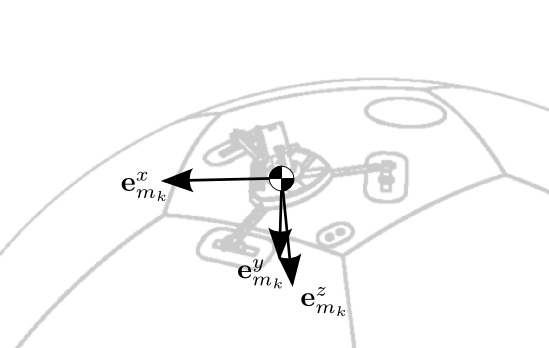
\includegraphics[scale=1]{images/tangential_frame.png}
\caption{The \textit{tangential frame} is the coordinate frame of the motor at its \textit{true} position. If the true position is not known, an estimate is used. In any case, its $\lbrace \mathbf{e}^x_{m_k} , \mathbf{e}^y_{m_k} \rbrace$ plane will be tangential to the spherical hull such that an error of the arrangement can be approximated by the euclidean norm in the tangential coordinate frame.}
\label{fig:tangential_frame}
\end{figure}

BLA BLA BLA
We recorded one large dataset.
Same inputs to simulation.
Split large datasets into multiple datasets ('normal' size) s.t. we have some statistics.

\section{Simulation}
To test our optimization framework, we defined five test cases.
\begin{itemize}
\item[Default] A simulation of Skye blimp that is comparable to the real Skye system. All 21 parameters as listed in \cref{tab:params_updated} are estimated.
\item[1 AU] As default, but only one of the AUs of Skye is estimated (AU 4). The remaining AUs are not powered at all. 12 parameters estimated.
\item[5 AU] Different Skye blimp with 5 AUs. Configuration for all AUs estimated. 24 parameters.
\item[No Drag] As default, but simulation without aerodynamic drag. This is used to see how much drag influences the result accuracy.
\item[COG] As default, but with large additional weight at AU4 position. COG to COB offset is 10cm and yields a moment in the same magnitude as the actuation moment. This is used to estimate the error introduced by large COG shifts.
\end{itemize}
\subsection{Estimation Confidence}

...Show estimate STD: BAR PLOTs.\\
...Similar explanations as in Presentation

\begin{figure}[hbtp]
\centering
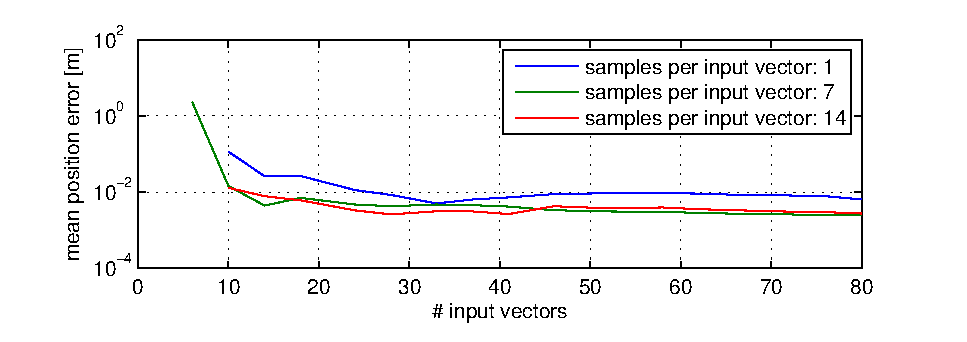
\includegraphics[width = \textwidth]{images/results/input_length_vs_position_error.eps}
\caption{Influence of the data set length on the mean position estimate error of the four AUs $e_{pos}$.}
\label{fig:result_inputlength}
\end{figure}

An important observation can be made about the influence of the dataset length on the estimate error.
\Cref{fig:result_inputlength} shows the change of error with increasing length of the dataset.
The more different input vectors are used for the batch optimization, the better gets the estimate.
When using multiple samples of the same input vector (in \cref{result_inputlength} shown for 1, 7, and 14 samples per input vector), the estimation error decreases as well.
It can be seen that considering multiples of the same input vectors alone is not sufficient, to get a better estimate.
Varying the input is at least that important.

\subsection{Convergence Regions}
The impact of the initial estimate for the batch optimization has been tested.
Using different a grid of different initial configuration estimates, the failure rate for different input realizations has been tested and is shown in \cref{fig:result_sim_convergece_region}.
It can be seen, that a initial position offset of \textit{all} motors in any random direction\footnote{
The simulated blimp has a hull radius of \unit[1.37]{m} and therefore the distance between two of the tetrahedrally arranged actuation units is \unit[2.62]{m}.}
is acceptable up to \unit[1]{m}.
Initial orientation offsets of the motors are acceptable up to \unit[120]{°}.
\\
The same observation can be made when using datasets from real measurements (compare \cref{fig:result_real_convergece_region}).
Further results using real measurements are showed in the next section.

\begin{figure}[hbtp]
\centering
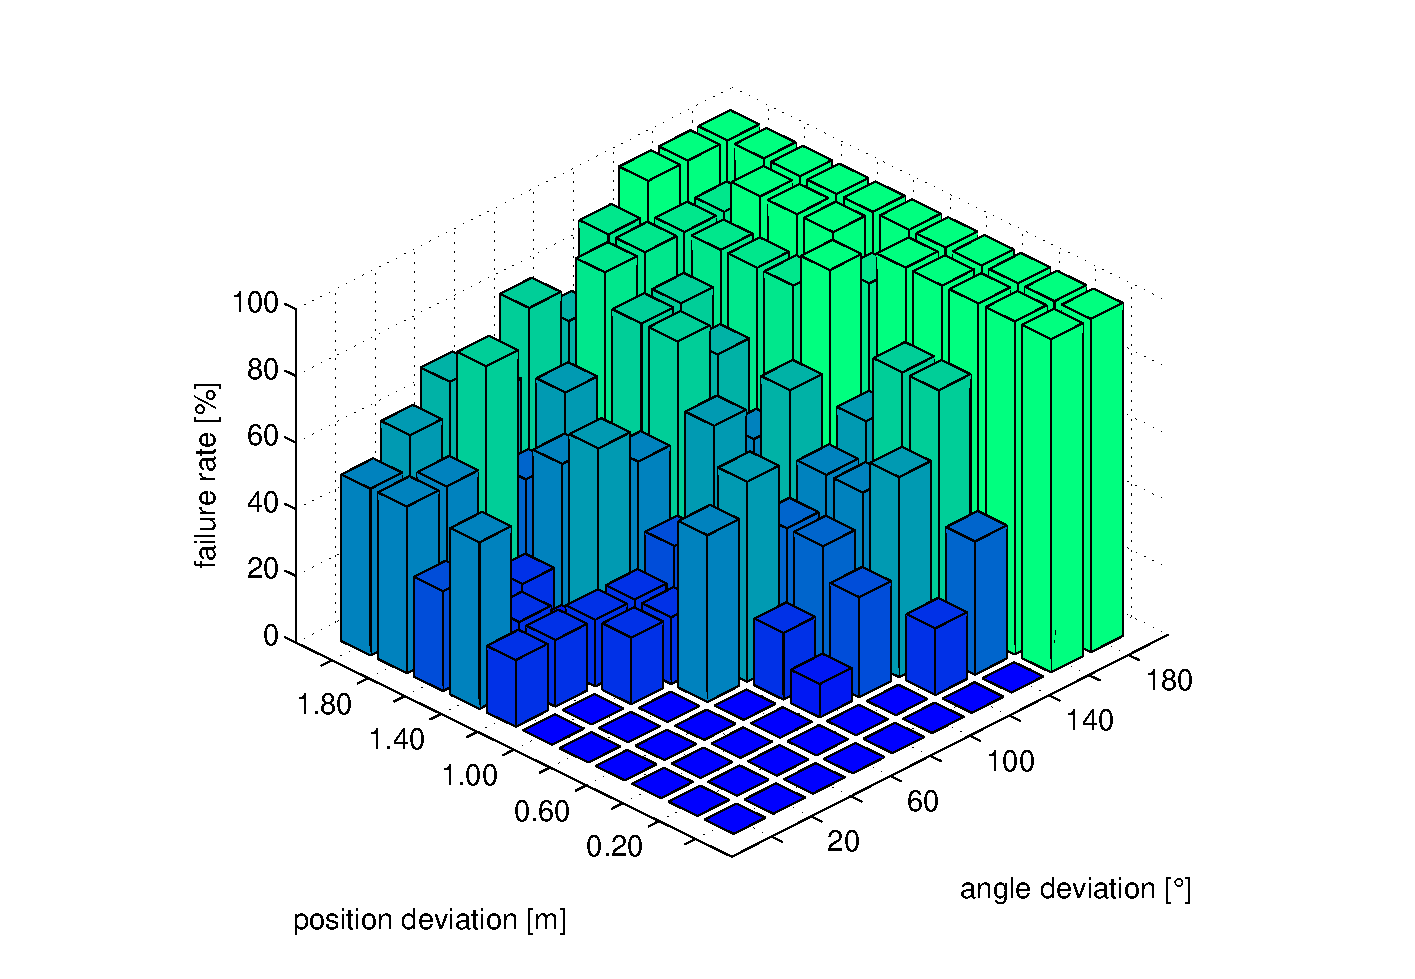
\includegraphics[width = \textwidth]{images/results/convergence_analysis_init_deviation_sim_bar.eps}
\caption{Failure rate using simulation data and different initial guess about actuation configuration.}
\label{fig:result_sim_convergece_region}
%\end{figure}
%
%\begin{figure}[hbtp]
\centering
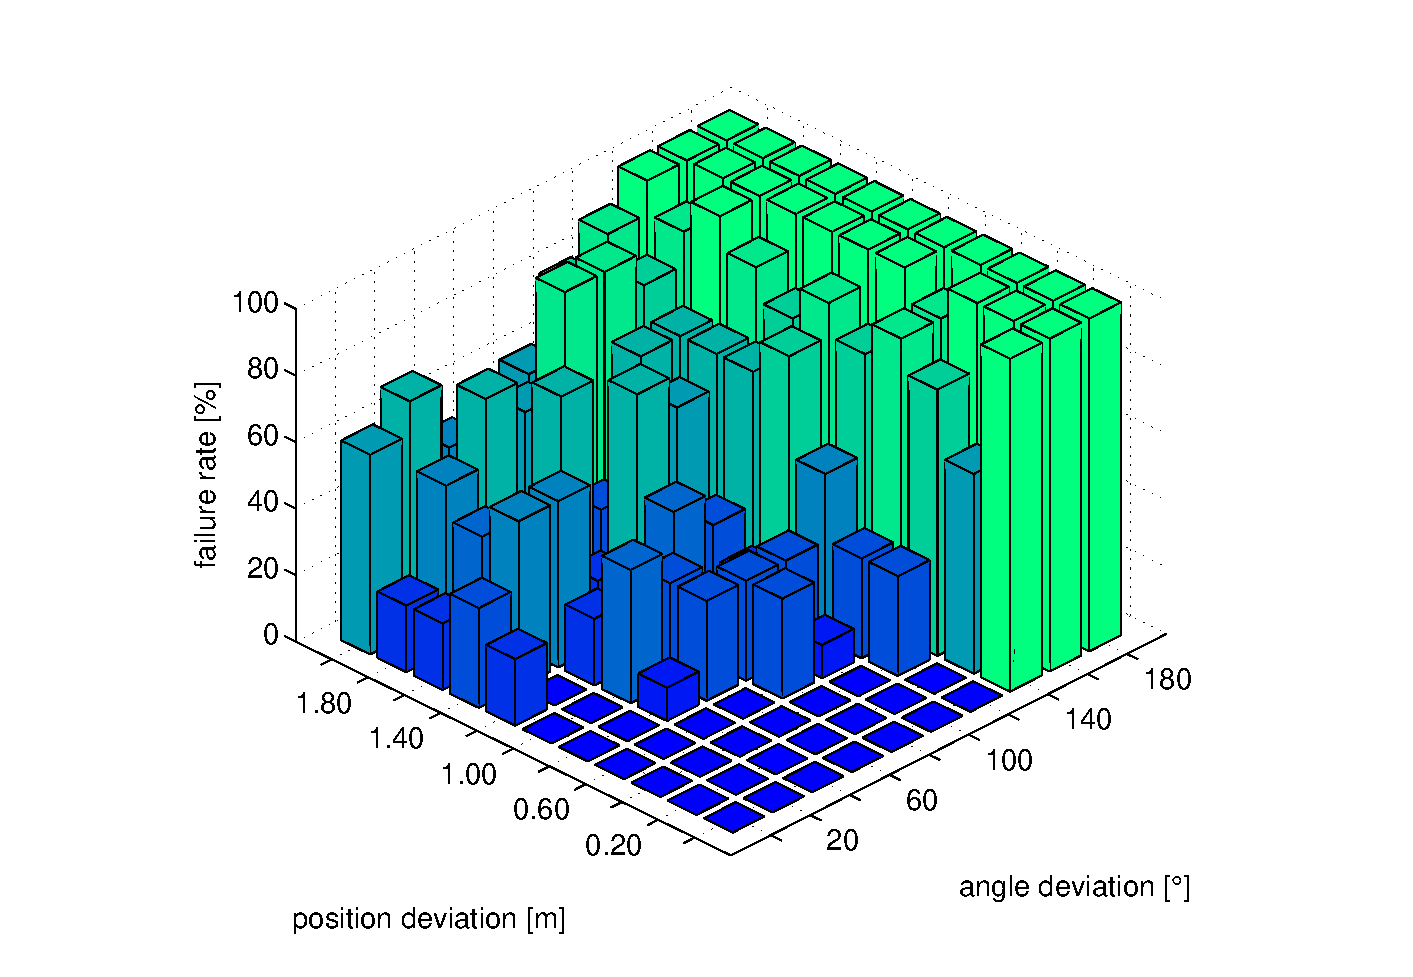
\includegraphics[width = \textwidth]{images/results/convergence_analysis_init_deviation_real_bar.eps}
\caption{Failure rate using experiment data and different initial guess about actuation configuration.}
\label{fig:result_real_convergece_region}
\end{figure}


\section{Experiments}
\subsection{Estimation Confidence}
...Copy past from Simulation. Replace STD by RMS. Compare Experiment with Simulation.
...That means do not show a 'you-know-which-plot' again (it will be very similar to the one above)
...But show this angular acceleration plot. Add a error subplot to it.
\subsection{Convergence Regions}
...Same as above
\section{Ground Truth}
...Do not tell toooo much in this section. Nobody likes to read long reports. So just mention 'we did it' and show the results.

...